% first example chapter
% @author Jan Robert Rösler 
%
\chapter{Entwurf}
In diesem Kapitel wird der vollständige Entwurf einer Steuerung für ein RC Fahrzeug dargestellt.

Wie im vorangegangenen Kapitel erläutert, entstand die Idee für die Steuerung eines RC-Fahrzeuges mit Neuronalen Netzen im Kontext einer Arbeit der ETH Zürich.
Das dort entworfene DroNet wurde bereits kurz vorgestellt und wird die Basis für die neuronale Steuerung sein. Zunächst sollen darum die technischen Aspekte von DroNet hervorgehoben werden: \\

DroNet ist ein 8-Layer Convolutional Neural Network, das insbesondere aus drei Residual-Blöcken besteht und für den Input eines 200x200 Pixel Bildes in Graustufen zwei Outputs produziert, einmal einen Lenkwinkel aus dem Intervall [-1,1] (hierbei gilt; Werte~<0 entsprechen einer Rechtskurve, Werte~>0 einer Linkskurve)  und einmal die Kollisionswahrscheinlichkeit in Prozent (als Klassifizierungsproblem in Prozentschritten, nicht kontinuierlich).\\
DroNet hat \num{3.2e5} Parameter und schafft eine Verarbeitungsrate von 20 fps ( Die Drohne, auf der DroNet getestet wurde lieferte Bilder mit 30 Hz).
Wie im vorigen Kapitel bereits erwähnt, wurde DroNet auf einem frei verfügbaren Datensatz trainiert. Im Paper werden dann Ergebnisse mit anderen Netzwerken verglichen, die mit dem selben Datensatz trainiert wurden, um die Performance zu Vergleichen. Ein solcher Vergleich ist für diese Arbeit jedoch nicht sinnvoll, da es um die Anwendung auf ein spezifisches, reales Szenario geht. 

\section{Hardware und Strecke}

Das vom HAW-Team aufgebaute Fahrzeug für den Carolo-Cup (Abbildung~\ref{img:Carolo-Fahrzeug} zeigt die Seitenansicht), besteht, abgesehen von Chassis, Motorelektronik und Servos, im Kern aus einem Intel NUC, auf dem die vollständige Bildverarbeitung und Logik berechnet wird und der Kamera, die die Bilder liefert (montiert an einem Alustab). Die Kamera ist eine \textsc{ueye} Schwarweißkamera der Firma IDS, die über USB mit dem NUC verbunden ist. 
Die Kontrolle per Fernsteuerung, zum Eingreifen im Fehlerfall und zum Positionieren des Fahrzeugs kommuniziert über Funk direkt mit dem Motorcontroller.\\
Auf dem Intel NUC ist ein Unix Betriebssystem eingerichtet.
Eine funktionsfähige Hardware Abstraktion für den Motor und die Steuerungsservos ist vom Carolo-Cup Team bereits entwickelt und steht mir im Weiteren zur Verfügung, diese ist in C++ implementiert.\\

\begin{figure}[h]
	\centering
	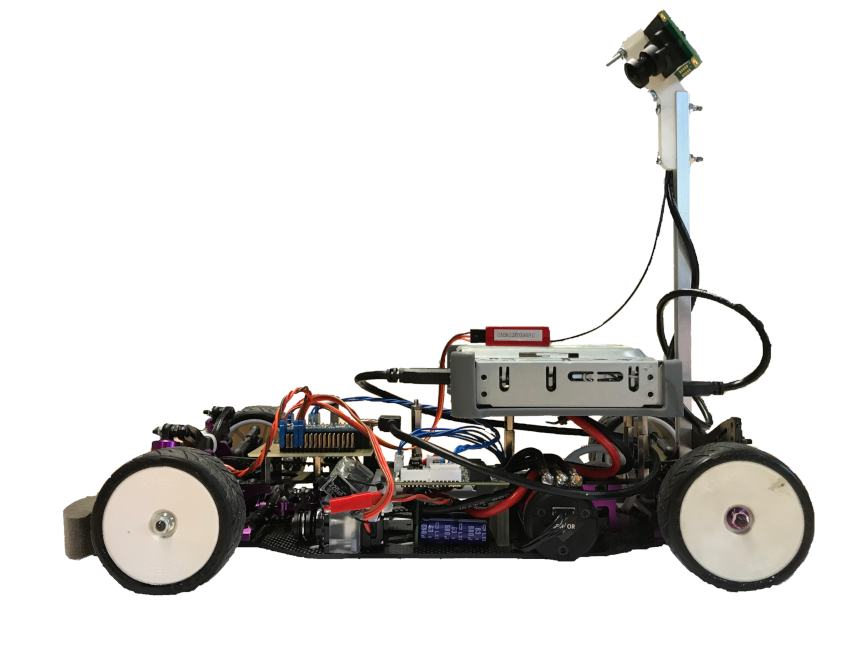
\includegraphics[scale=0.3]{figures/Fahrzeug.png}
	\caption{Das Carolo-Cup Fahrzeug}
	\label{img:Carolo-Fahrzeug}
\end{figure}

Die Teststrecke, die an der HAW zur Verfügung steht, ist ein Rundkurs mit verschiedenen Kurven und einem Kreuzungszenario \note{Collage mit Bildern}. Die Länge der äußeren Fahrbahn beträgt 36,1 Meter, die innere Fahrbahn ist 31,3 Meter lang.\\
Die Fahrbahn mit weißen Band auf schwarzem Untergrund abgeklebt und entspricht der Erscheinung einer Straße, mit unterbrochener Mittellinie. Einige Besonderheiten der Strecke, wie zum Beispiel Parklücken, sind Teil der Aufgaben des Carolo-Cups, spielen in dieser Arbeit aber keine Rolle.
Die Abbildung~\ref{img:teststrecke} zeigt einen Ausschnitt der Fahrbahn, zu sehen ist eine fast kreisförmige Kurve und die Kreuzungssituation. 
Der Teststreckenraum ist fensterlos, es wurde sowohl bei Aufnahme der Trainingsbilder, als auch bei den Testfahrten darauf geachtet, dass die volle Deckenbeleuchtung an ist, um für optimale und gleichbleibende Beleuchtungsverhältnisse zu sorgen.

\begin{figure}[h]
	\centering
	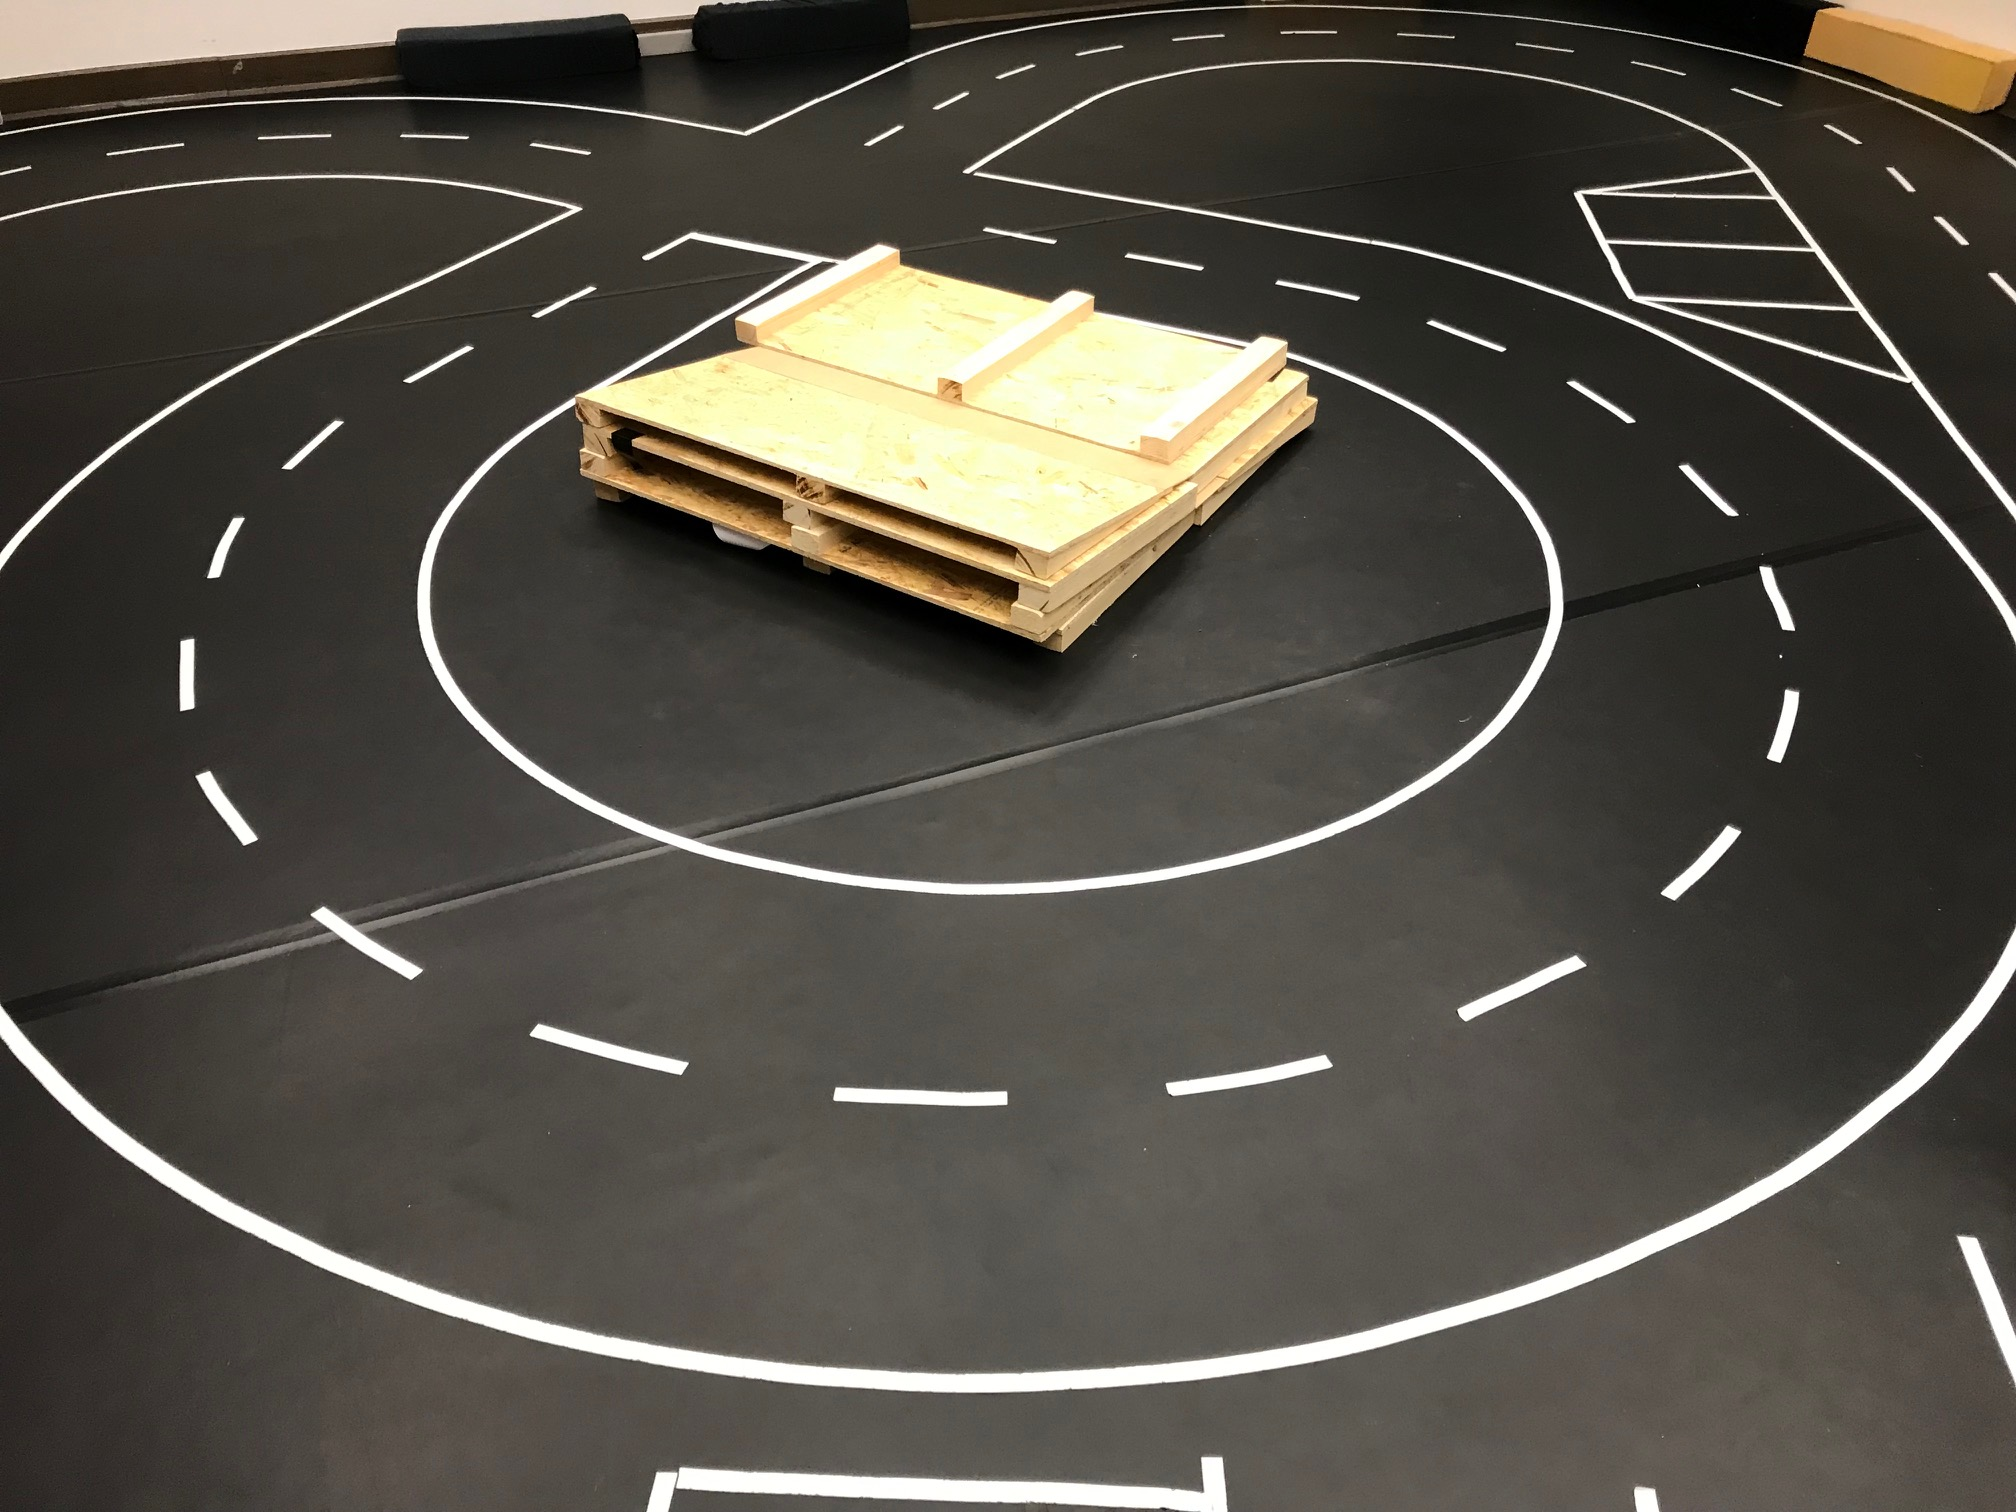
\includegraphics[scale=0.2]{figures/Teststrecke-Ausschnitt.jpg}
	\caption{Ein Ausschnitt der Teststrecke}
	\label{img:teststrecke}
\end{figure}

Bildverarbeitung und Training des Netzes werden auf einem Windows Computer mit einer GeForce GTX 950 Grafikkarte berechnet. Da mit einer relativ kleinen Bildanzahl gearbeitet wird und das Neuronale Netz sehr kompakt ist, wird keine High-end Grafikkarte benötigt.


\section{Trainingsdaten}

Um Trainingsdaten, also Bilder der Teststrecke mit dazugehörigem Lenkwinkel zu bekommen, wird auf einen Algorithmus eines Carolo-Cup Teams (TeamWorstCase) der HAW zurückgegriffen. Trainingsdaten per Hand zu generieren erwies sich als sehr schwierig, per Fernsteuerung lässt sich kaum sauber und kontinuierlich durch den Rundkurs steuern.\\
Auf mehreren Fahrten über den Rundkurs mit dem Algorithmus von Team \textsc{TeamWorstCase}, wurden über 20.000 Bilder gesammelt. Da die Steuerung nicht völlig sauber funktionierte und die Bildfolgen mehrfach Ausreisser enthielten, mussten Bilder per Hand aussortiert werden. Am Ende dieser Vorauswahl standen etwas über 6000 Bilder für das Training zur Verfügung. Die Auflösung der Aufnahmen ist 752x480 Pixel. Die untere Hälfte der Bilder ist durch eine kamerainterne Vorverarbeitung bereits geschwärzt, Team \textsc{TeamWorstCase} hat für ihre weitere Verarbeitung so direkt den Teil des Bildes ausgeblendet, auf dem das Fahrzeug selbst zu sehen ist. Da dieser Teil des Bildes im weiteren ohnehin weggeschnitten wird, hat das keine Auswirkungen. \\
Ein Beispiel aus diesen Fahrbahnaufnahmen zeigt Abbildung~\ref{img:rohbild}, die Aufnahme ist automatisch in Graustufen, da die Kamera nur in diesem Farbmodus aufnimmt.
Diese Rohdaten sind die Basis für das Training und müssen dazu einer Vorverarbeitung unterzogen werden. 

\begin{figure}[h]
	\centering
	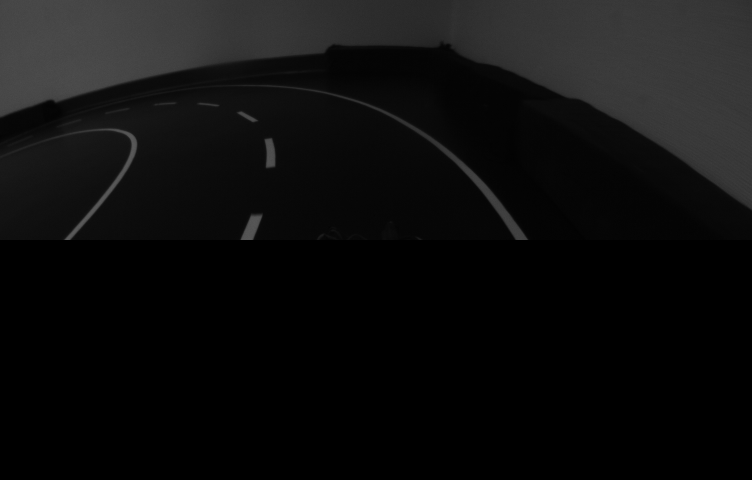
\includegraphics[scale=0.4]{figures/Rohbild.png}
	\caption{Kameraaufnahme der Fahrbahn}
	\label{img:rohbild}
\end{figure}


\section{Vorverarbeitung und Fine Tuning}

\subsection{Software}
Die Bildverarbeitung und das Training sind mit Python programmiert. Für Operationen auf Bildern wird die OpenCV Bibliothek verwendet. Das Neuronale Netz und die Struktur für Verarbeitung der Bilder und Training sind mit Keras implementiert.\\
Einzelne Funktionen zur Auswertung und für das Training sind aus dem Repository der DroNet Gruppe der ETH Zürich übernommen, diese sind im Code entsprechend kenntlich gemacht.\\
Die Abstraktion für den Motorcontroller auf dem Fahrzeug ist in C++ implementiert, die Steuerungskontrolle auf Fahrzeugseite ist daher in C entwickelt.\\
Die Python Module laufen auf einem Windows Computer in einer virtuellen Umgebung, die mit Anaconda verwaltet wird. Es sind 2 Umgebungen mit Python 3.6.5 eingerichtet. Auf dem Fahrzeug (NUC) kommt zusätzlich Visual Studio Code zum Einsatz, so wie eine Debugging Umgebung mit PyCharm für die Python Module.

\subsection{Preprocessing}
Um die Bilder für das Training aufzubereiten, wird eine Verarbeitungspipeline eingerichtet, die in der gleichen Form auch für die Vorverarbeitung im Steuerungsmodus genutzt wird. Die Bilder, die das Netz zum Training zu \glqq sehen \grqq{} bekommt, sollen die gleiche Verarbeitung durchlaufen wie die Live-Bilder, die später zum Steuern benutzt werden.


\begin{figure}[h]
	\centering
	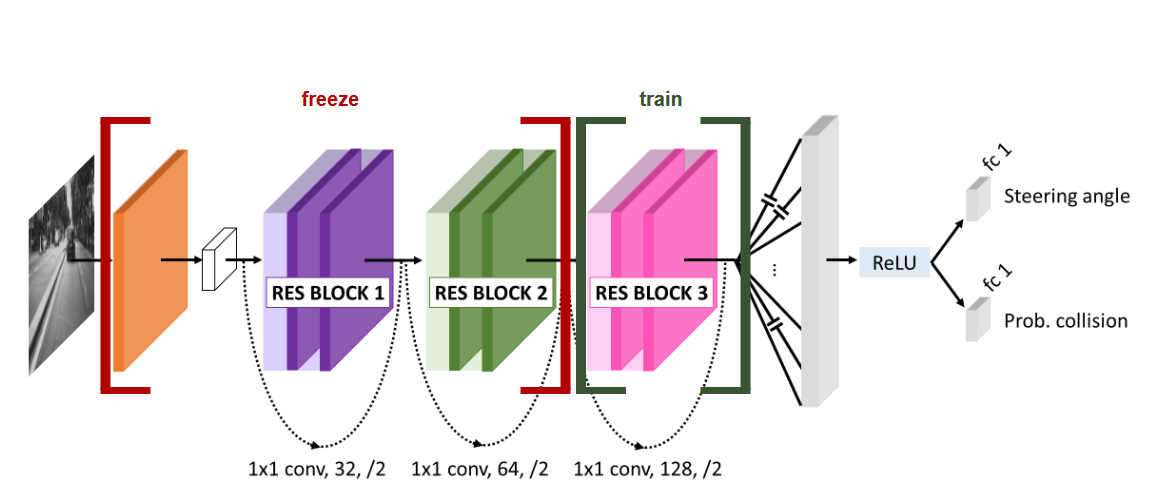
\includegraphics[scale=0.5]{figures/Architecture-DRONET-FROZEN.png}
	\caption{Angepasste Architektur}
	\label{img:dronetfrozen}
\end{figure}



Adaption auf das Carolo Cup Fahrzeug

GRUNDSATZ: , Chollet depp learning zitieren

\subsection{Fine Tuning}

\note{Hervorhaben, welche Teile des DroNet Codes ich weiterverwede. Hard Mining, Auswertungsfunktionen, Architektur}

Änderungen an der Architekrtur des Netzes
Lernarchitekrur (Pipepline)
Steuerungsarchitektur
Bilder mit Steuerdaten (Verarbeitungspipeline) UND VERDOPPELUNG DER DATEN
Fahrzeug (Kamera, Rechner etc.)

Training 
Performance (Rechenzeit) bei prediction auf dem Fahrzeug
Kommunikation zwischen C und pYthon

\note{BILD der STrecke}

\section{Steuerung}

Kamerakonfiguration
Steuerungskomponenten
Kommunikation C++/Python



Kurzer Blick auf  Self driving car steering angle4 prediction und berkeley (large scale video sets) (vielleicht auchSPÄTER)

